\documentclass[11pt]{article}
\usepackage[ngerman]{babel}
\usepackage{tocloft}
\usepackage{titlesec}
\usepackage{etoolbox}
\usepackage{setspace}
\usepackage{graphicx}
\usepackage{enumitem}
\usepackage{tcolorbox}
\usepackage[skip=0.5em]{caption}
\usepackage[left=2cm, right=2cm, top=2cm, bottom=2cm]{geometry}

\renewcommand*\contentsname{Inhaltsverzeichnis} %defines the name of the toc
\renewcommand*\thesection{2.\arabic{section}} %defines a custom numbering for sections

% sets new length variable, only used for custom environment
\newlength{\subsectionindent}
\setlength{\subsectionindent}{4.2em}
\newlength{\reflexionindent}
\setlength{\reflexionindent}{2.2em}

%defines an environment that applies a custom indent to text inside
\newenvironment{subindent}[1][\subsectionindent]
{%
  \begingroup
  \setlength{\leftskip}{#1}%
  \setlength{\parindent}{0pt}%
}
{%
  \par\endgroup
}

%defines an environment that applies a custom indent to text inside
\newenvironment{refindent}[1][\reflexionindent]
{%
  \begingroup
  \setlength{\leftskip}{#1}%
  \setlength{\parindent}{0pt}%
}
{%
  \par\endgroup
}

\begin{document}

% applies a custom font and layout to sections
\titleformat{\section}
  {\normalfont\Large\bfseries}
  {\thesection}{0.5em}{}
\titlespacing*{\section}{0em}{*3}{*1}

% applies a custom font and layout to subsections
\titleformat{\subsection}
  {\normalfont\large\bfseries} % font
  {\thesubsection}{0.5em}{} % section number and space between num and title
\titlespacing*{\subsection}{1em}{*2}{*0.5} % spacing around titles

% forces a fixed indent for EVERYTHING (applies to formatting of boxes and img)
% \makeatletter
% \pretocmd{\subsection}{\setlength{\leftskip}{4.2em}}{}{}
% \pretocmd{\section}{\setlength{\leftskip}{0pt}}{}{}
% \makeatother

\begin{titlepage}
    \begin{center}
        \vspace*{1cm}
        \LARGE
        Lernfeld 2 Portfolio

        \vspace{0.5cm}
        \Huge
        \textbf{Arbeitsplätze nach Kundenwunsch ausstatten}

        \vspace{1.5cm}
        \large
        %\textbf{Christopher Vitz}

        \vspace*{\fill}
        Technisch-Gewerbliches Berufsbildungszentrum Saarbrücken \\
        \today
    \end{center}  
\end{titlepage}

{
\fontsize{12pt}{12.5pt}\selectfont
\cftsetindents{section}{0em}{2.5em}
\cftsetindents{subsection}{1em}{3em}
%toc in need of formatting (line spacing, font size)
\tableofcontents
}

\newpage
\section{Eine Einführung in die IT für Arbeitsplätze geben}
\subsection{Eine Einführung in Grundfunktionen des Computers geben}
    \vspace{0.5em}
    \begin{tcolorbox}[width=9cm, center, title=EVA-Grundprinzip der Datenverarbeitung, coltitle=white, colframe=orange, colback=white!60!orange]
        \begin{itemize}
            \item[E =] Eingabe
            \item[V =] Verarbeitung
            \item[A =] Ausgabe
        \end{itemize}
    \end{tcolorbox}
    \vspace{-0.5em}
    \begin{figure}[h]
        \centering
        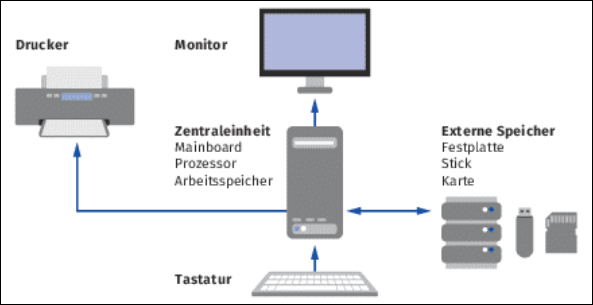
\includegraphics[width=0.7\textwidth]{./images/2.1.1_konfiguration.png}
        \caption{EVA-Prinzip Beispiel}\label{fig:EVA-Prinzip}
    \end{figure}
    \vspace{-0.5em}
    \begin{tcolorbox}[width=13cm, center, title=Konfiguration, coltitle=white, colframe=white!20!blue, colback=white!80!blue]
        Bezeichnung für abgestimmte Zusammenstellung von Hardware und Software auf Nutzungszweck des Kunden.
    \end{tcolorbox}
    \vspace{0.25em}
\subsection{Bedeutende Entwicklungsschritte in der Computertechnik}
    \vspace{0.5em}
    \begin{itemize}[leftmargin=3cm]
        \item[1980er:] IBM, 8Bit Prozessor, 64KB RAM
        \item[1990er:] Open Source, Internet, Google
        \item[2000er:] Open Office, Facebook
        \item[2020er:] KI, 64Bit Prozessor, 64GB+ RAM
        \item[2030er:] Quantencomputer
    \end{itemize}

\newpage
\subsection{Entwicklungstrends präsentieren}
    \vspace{-0.5em}
    \begin{figure}[h]
        \centering
        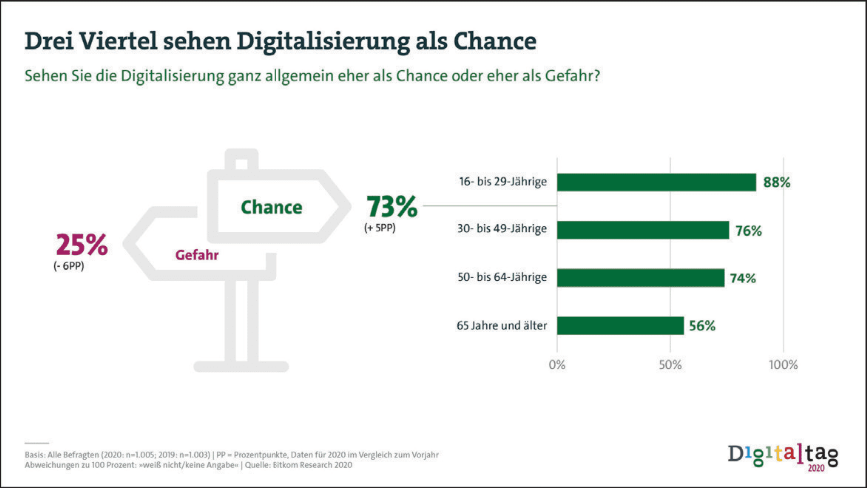
\includegraphics[width=0.7\textwidth]{./images/2.1.3_entwicklungstrend-digitalisierung.png}
        \caption{Entwicklungstrend zur Digitalisierung}\label{fig:Entwicklungstrend_Digitalisierung}
    \end{figure}
    \vspace{-0.5em}
\subsection{Komponentenhersteller und Systemarchitekturen präsentieren}
    \begin{subindent}
        Wichtige Hersteller in der heutigen Zeit:
    \end{subindent}
    \vspace{-0.5em}
    \begin{itemize}[leftmargin=2.5cm]
        \item Intel (Prozessor Marktführer)
        \item AMD (Konkurrent zu Intel)
        \item NVIDIA (Größter Grafikkartenentwickler)
        \item ARM (Prozessorarchitektur)
        \item Apple
        \item Microsoft (Betriebssystem Marktführer)
    \end{itemize}
    \vspace{0.5em}
    \begin{tcolorbox}[width=15cm, center, title=Kompatibilität, coltitle=white, colframe=white!20!blue, colback=white!80!blue]
        Bezeichnung für Verträglichkeit von Komponenten zeinander.
        \begin{itemize}[labelsep=1em, align=parleft, leftmargin=*, widest=Abwärtskompabilität, itemsep=0em]
            \item[Aufwärtskompabilität:] Vorgängerversionen funktionieren mit Nachfolgeversionen
            \item[Abwärtskompabilität: ] neuere Komponenten funktionieren mit Vorgängerversionen
        \end{itemize}
    \end{tcolorbox}
\subsection*{Reflexion Kapitel 2.1}
\addcontentsline{toc}{subsection}{Reflexion Kapitel 2.1}
    \begin{refindent}
        Grundlage zur Verbindung der einzelnen Komponenten eines Computers erlernt (EVA-Prinzip, Konfiguration und Kompatibilität).
        Ebenso ein grobes Wissen über die Entwicklung der IT erlangt, mit möglichen zukünftigen Entwicklungen.
        Verschiedene Hersteller kennengelernt, die einen Großteil des Marktes ausmachen.
    \end{refindent}

\newpage
%TODO Formatting
\section{Das Leistungsportfolio im Ausbildungsbetrieb präsentieren}
\subsection{Arbeitsplätze und Arbeitsumgebungen für IT-Systeme beschreiben}
    \begin{subindent}
        IT ist heutzutage sowohl im privaten sowie industriellen Kontext nicht wegzudenken. \\
        Einsatzbereiche der IT:
    \end{subindent}
    \begin{itemize}[leftmargin=2.5cm, topsep=0.3em, itemsep=0.1em, parsep=0.5em]
        \item Privat
        \item Industrie
        \item Wirtschaft
        \item Verwaltung
    \end{itemize}
    \begin{subindent}
        Formen von Arbeitsarten:
    \end{subindent}
    \begin{itemize}[leftmargin=2.5cm, topsep=0.3em, itemsep=0.1em, parsep=0.5em]
        \item Telearbeiten: Arbeiten an einem eingerichteten Arbeitsplatz
        \item mobiles Arbeiten: auch Homeoffice, Arbeit nicht an festen Arbeitsplatz gebunden
    \end{itemize}
    \begin{subindent}
        Die Arbeitsplätze dieser Arten sind nach Bürokonzepten gestaltet und müssen ergonomische, ökologische und gesundheitliche Anforderungen berücksichtigen. \\
        Formen von Arbeitsumgebungen:
    \end{subindent}
    \begin{itemize}[leftmargin=2.5cm, topsep=0.3em, itemsep=0.1em, parsep=0.5em]
        \item Zellenbüros: Ein-/Mehrpersonenbüros entlang eines FLurs
        \item Großraumbüros: Open-Space-Bürolandschaft
        \item Kombibüro: Einzelbüros entlag der Fassade, Pausenraum dazwischen
        \item Non-Territoriales Büro: Büroplätze werden von Mitarbeitern für Arbeitszeit gebucht
    \end{itemize}
    \begin{subindent}
        Bei der Gestaltung der Arbeitsplätze muss auf genügend Beleuchtung (min. 500 Lux) sowie eine nicht zu hohe Lärmentwicklung (30-45dB) geachtet werden.
    \end{subindent}
\subsection{Marktgängige IT-Systeme vorstellen}
    \begin{tcolorbox}[width=15cm, center, title=Konfiguration, coltitle=white, colframe=orange, colback=white!60!orange]
        Bezeichnung für die Zusammenstellung, Einstellung und Abstimmung von Komponenten/Geräten/Programmen in Bezug auf Anwendung. \\
        Unterscheidung vom Istzustand (Ist-Konfiguration) als aktuellem Stand und Sollzustand (Soll-Konfiguration) als Zielzustand.
    \end{tcolorbox}
    %TODO evtl die verschiedenen bauformen adden
    \vspace{-1em}
    \begin{figure}[h]
        \centering
        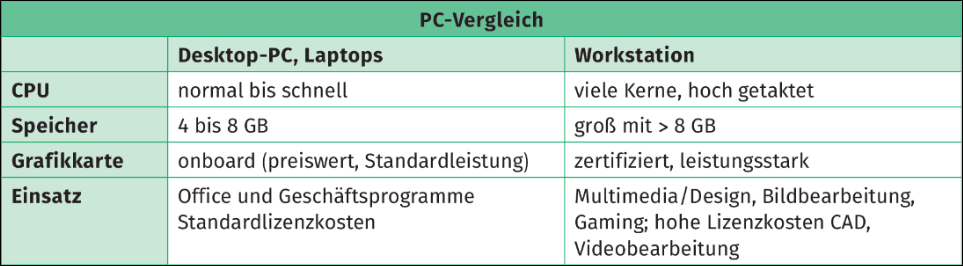
\includegraphics[width=0.7\textwidth]{./images/2.2.2_pc-vergleich.png}
        \caption{Unterscheidung der Leistungsfähigkeit}\label{fig:Leistungsfähigkeit_Unterscheidung}
    \end{figure}
    \begin{subindent}
        IT-Hardware kann auf verschiedene Kriterien und Spezifikationen geprüft werden. \\
        Dabei sind die folgenden von besonderer Bedeutung:
    \end{subindent}
    \begin{itemize}[leftmargin=2.5cm, topsep=0.3em, itemsep=0.1em, parsep=0.5em]
        \item Quantitative Größen (messbare, objektive Größen)
        \item Qualitative Größen (schwer messbare, subjektive Größen)
        \item Vergleiche (Stress-/Benchmarktests, etc.)
    \end{itemize}
    \begin{subindent}
        Desweiteren können zusätzliche Recherchen durchgeführt werden, etwa über das Internet (Fachportale, Blogs, etc.) oder Hardware-Tests und Diagnosetools.
    \end{subindent}
\subsection{Das Leistungsportfolio im IT-Bereich präsentieren}
    \begin{subindent}
        Das Leistungsportfolio eines Unternehmens beschreibt die Dientsleistungen und Tätigkeiten eines Betriebs. \\
        Bei Unternehmen mit interner IT, ist die IT-Abteilung der Dienstleister der Mitarbeiter und Abteilungen. Die Mitarbeiter sind demnach interne Kunden.
    \end{subindent}
\subsection*{Reflexion Kapitel 2.2}
\addcontentsline{toc}{subsection}{Reflexion Kapitel 2.2}
    %TODO REFLEXION
    \begin{refindent}
        TODO
    \end{refindent}

\newpage
\section{Auswahlkriterien zu IT-Produkten allgemein unterscheiden}
\subsection{Qualität und Leistungsfähigkeit von IT-Systemen und IT-Services beschreiben}
    TODO
\subsection{Umweltschutz und Green-IT als wichtige IT-Ziele darstellen}
    TODO
\subsection{Wirtschaftlichkeit von IT-Systemen erläutern}
    TODO
\subsection{IT-Sicherheit von IT-Systemen, Informations- und Datenschutz erläutern}
    TODO
\subsection*{Reflexion Kapitel 2.3}
\addcontentsline{toc}{subsection}{Reflexion Kapitel 2.3}
    %TODO REFLEXION
    \begin{refindent}
        TODO
    \end{refindent}

\newpage
\section{Komponenten eines Arbeitsplatzcomputers unterscheiden}
\subsection{Zentraleinheit, Mainboard und Betriebssystem unterscheiden}
    TODO
\subsection{Hauptplatine, Mainboard und die Komponenten unterscheiden}
    TODO
\subsection{Prozessoren genauer beschreiben}
    TODO
\subsection{Arbeistspeicher (RAM-Speicher) erläutern}
    TODO
\subsection{Schnittstellen und Anschlüsse am Mainboard erläutern}
    TODO
\subsection{Netzteile beschreiben und unterscheiden}
    TODO
\subsection{Festplatten unterscheiden und erläutern}
    TODO
\subsection{Tastaturen unterscheiden und präsentieren}
    TODO
\subsection{Monitore vergleichen und präsentieren}
    TODO
\subsection{Leistungsmerkmale für Drucker und Zusatzanforderungen erläutern}
    TODO
\subsection{Scanner beschreiben und für Arbeitsplatz auswählen}
    TODO
\subsection{IT-Zubehör für die Barrierefreiheit und im Aftersales unterscheiden}
    TODO
\subsection{Unternehmenssoftware anbieten und vergleichen}
    TODO
\subsection{Marktgängige IT-Systeme und Lösungen anbieten}
    TODO
\subsection*{Reflexion Kapitel 2.4}
\addcontentsline{toc}{subsection}{Reflexion Kapitel 2.4}
    %TODO REFLEXION
    \begin{refindent}
        TODO
    \end{refindent}

\newpage
\section{Kundenanforderungen im Leisuntgsprozess berücksichtigen und Projektmanagement vorbereiten}
\subsection{Anforderungen zur Kundenzufriedenheit in den Leistungsprozess einbeziehen}
    TODO
\subsection{Marketing- und Verkaufsförderungsmaßnahmen unterstützen}
    TODO
\subsection{Auftragsbearbeitung mit Projektmanagement unterstützen}
    TODO
\subsection*{Reflexion Kapitel 2.5}
\addcontentsline{toc}{subsection}{Reflexion Kapitel 2.5}
    %TODO REFLEXION
    \begin{refindent}
        TODO
    \end{refindent}

\newpage
\section{Bedarfs- und Anforderungsanalysen durchführen}
\subsection{Den Prozess der Anforderungsanalyse erläutern}
    TODO
\subsection{Kundenanforderungen formulieren}
    TODO
\subsection{Hardware- und Systemvorraussetzungen prüfen}
    TODO
\subsection*{Reflexion Kapitel 2.6}
\addcontentsline{toc}{subsection}{Reflexion Kapitel 2.6}
    %TODO REFLEXION
    \begin{refindent}
        TODO
    \end{refindent}

\newpage
\section{Pflichtenhefte erstellen}
\subsection{Anforderungsanalysen zu Desktops und Workstations durchführen}
    TODO
\subsection{Anforderungsanalysen zu Laptops und Tablets durchführen}
    TODO
\subsection{Anforderungsanalysen zu Thin Clients durchführen}
    TODO
\subsection{Desktop as a Service, Miete, Finanzierung und Leasing als Dientsleistungen berücksichtigen}
    TODO
\subsection*{Reflexion Kapitel 2.7}
\addcontentsline{toc}{subsection}{Reflexion Kapitel 2.7}
    %TODO REFLEXION
    \begin{refindent}
        TODO
    \end{refindent}

\newpage
\section{Angebote und Stundensätze kalkulieren und die Rendite berücksichtigen}
\subsection{Beschaffungsprozess und Beschaffungsplanung erläutern}
    TODO
\subsection{Quantitative Angebotsvergleiche vornehmen}
    TODO
\subsection{Nutzwertanalysen durchführen}
    TODO
\subsection{Vertragsarten und AGB unterscheiden}
    TODO
\subsection*{Reflexion Kapitel 2.8}
\addcontentsline{toc}{subsection}{Reflexion Kapitel 2.8}
    %TODO REFLEXION
    \begin{refindent}
        TODO
    \end{refindent}

\newpage
\section{Lieferung, Installation und Übergabe vornehmen}
\subsection{Vorbereitung der Abnahme von Produkten und Leistungen}
    TODO
\subsection{Arbeitssicherheit und Gesundheitsschutz bei der Arbeit gewährleisten}
    TODO
\subsection{Für IT-Sicherheit am Arbeitsplatz eine Risikoanalyse vorbereiten}
    TODO
\subsection{Abfall- und Recyclinggesetze beachten}
    TODO
\subsection{Systemlieferung, -installation und -übergabe als Prozess präsentieren}
    TODO
\subsection*{Reflexion Kapitel 2.9}
\addcontentsline{toc}{subsection}{Reflexion Kapitel 2.9}
    %TODO REFLEXION
    \begin{refindent}
        TODO
    \end{refindent}

\newpage
\section{Kontrolle und Reflexion von Unterricht und betrieblicher Mitarbeit}
    TODO

\end{document}